\documentclass[xcolor=pdftex,dvipsnames,table,mathserif]{beamer}
%\usepackage{subfigure}
\usepackage{amsbsy}
\usepackage{tikz}
\usetikzlibrary{arrows}
\usepackage{amsmath,graphicx,dsfont,color}
\usepackage{amsfonts}
\usepackage{amssymb}
\usepackage{array}

\usepackage{subfig}

% makes the subfig package work
\makeatletter
\let\@@magyar@captionfix\relax
\makeatother

% subfigure counter resets every frame
\makeatletter
\@addtoreset{subfigure}{framenumber}
\makeatother

% First author and year
\bibliographystyle{apalike}

% This sets the list items of the bibliography to the same symbol used for citation.
\setbeamertemplate{bibliography item}{\insertbiblabel}

% This avoids extralines for different entries
\setbeamertemplate{bibliography entry title}{}
\setbeamertemplate{bibliography entry location}{}
\setbeamertemplate{bibliography entry note}{}

\DeclareMathOperator*{\argmin}{arg\,min}
\DeclareMathOperator*{\argmax}{arg\,max}
%Definitiona

\newcommand{\x}{\mathbf{x}}
\newcommand{\X}{\mathbf{X}}
\newcommand{\W}{\mathbf{W}} %Weight
\newcommand{\bais}{\mathbf{b}}%Bais
\newcommand{\act}{\texttt{g}}%Activation
\newcommand{\loss}{L}
\newcommand{\pdata}{\hat{p}_{\texttt{data}}}
\newcommand{\nsize}{N}
\newcommand{\nfeatures}{P}
\newcommand{\param}{\boldsymbol{\theta}}
\newcommand{\featmap}{\boldsymbol{\phi}}
\newcommand{\EV}{\mathbb{E}}







\usepackage{physics}

\graphicspath{{../graphics/}}

\AtBeginSection[]{
  \begin{frame}{Contents}
    \tableofcontents[currentsection, hideothersubsections]
  \end{frame}
}

\AtBeginSubsection[]{
  \begin{frame}{Contents}
    \tableofcontents[currentsection, subsectionstyle=show/shaded/hide]
  \end{frame}
}

\setbeamertemplate{footline}[frame number]{}
\setbeamertemplate{navigation symbols}{}
\setbeamertemplate{section in toc}[square]
\setbeamertemplate{items}[square]

%% For image credits on image bottom right
\usepackage[absolute,overlay]{textpos}
\setbeamercolor{framesource}{fg=gray}
\setbeamerfont{framesource}{size=\tiny}
\newcommand{\source}[1]{\begin{textblock*}{4cm}(8.7cm,8.6cm)
    \begin{beamercolorbox}[ht=0.5cm,right]{framesource}
      \usebeamerfont{framesource}\usebeamercolor[fg]{framesource} Credits: {#1}
    \end{beamercolorbox}
\end{textblock*}}

\title{Unsupervised anomalous image detection}
\author{E. Decencière}
\date{MINES ParisTech\\
  PSL Research University\\
  Center for Mathematical Morphology
}
\titlegraphic{
\includegraphics[height=1.7cm]{../graphics/logoemp}}

\useinnertheme{rounded}
\usecolortheme{rose}

%%%%%%%%%%%%%%%%%%%%%%%%%%%%%%%%%%%%%%%%%%%%%%%%%%%%%%%
%%%%%%%%%%%%%%%%%%%%%%%%%%%%%%%%%%%%%%%%%%%%%%%%%%%%%%%

\begin{document}

\frame{\titlepage}

\frame{
  \frametitle{Contents}
  \tableofcontents[hidesubsections]
}

%%%%%%%%%%%%%%%%%%%%%%%%%%%%%%%%%%%%%%%%%%%%%%%%%%
%%%%%%%%%%%%%%%%%%%%%%%%%%%%%%%%%%%%%%%%%%%%%%%%%%
\section{Introduction}

%%%%%%%%%%%%%%%%%%%%%%%%%%%%%%%%%%%%
\begin{frame}{Definition in layman terms}


  \begin{block}{Anomaly detection}
  Let us consider a given set of images. Among these, some  are defined as being \alert{normal}. The aim of the detection task is to decide, for a given image, if it is normal, or not.

  The definition of normal images is given through a set of examples.
  \end{block}

  \begin{itemize}
  \item We will focus on images, but the problem is very general.
  \item We will suppose that we only have examples of normal images, i.e. that we are in a \alert{unsupervised} context. We assume that examples of anomalies are not representative enough or unknown.
  \end{itemize}



\end{frame}

%%%%%%%%%%%%%%%%%%%%%%%%%%%%%%%%%%%%
\begin{frame}{Example - set of normal images}

\begin{figure}[ht]
  \centering
  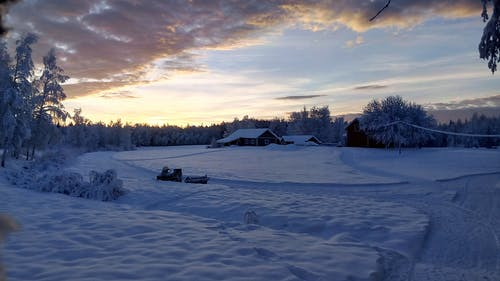
\includegraphics[width=0.3\textwidth]{snow1-pexels-photo-290548.jpg}
  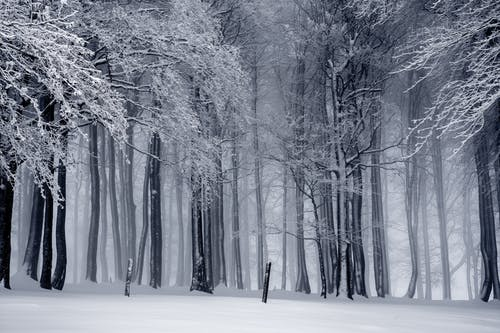
\includegraphics[width=0.3\textwidth]{snow2-pexels-photo-235621.jpg}
  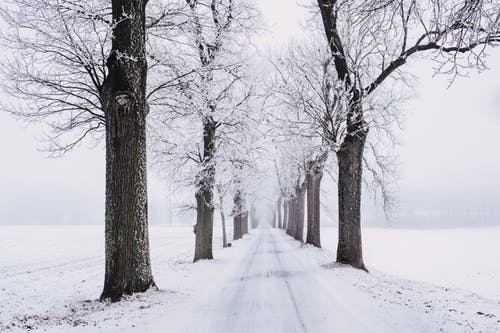
\includegraphics[width=0.3\textwidth]{snow3-pexels-photo-839462.jpeg}
  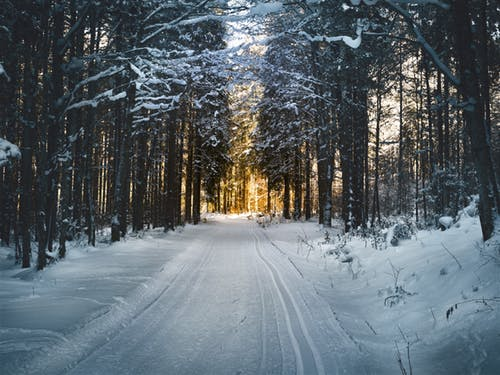
\includegraphics[width=0.3\textwidth]{snow4-pexels-photo-688660.jpeg}
  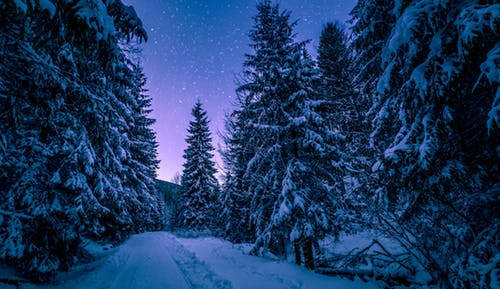
\includegraphics[width=0.3\textwidth]{snow5-pexels-photo-773594.jpeg}
  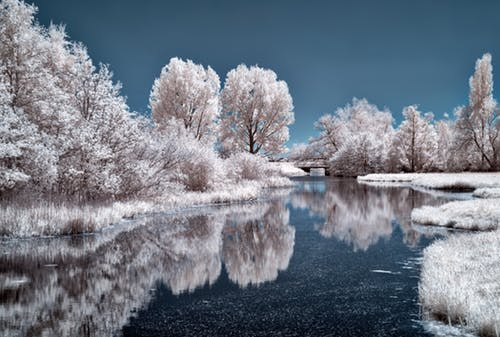
\includegraphics[width=0.3\textwidth]{snow6-pexels-photo-1559117.jpeg}
  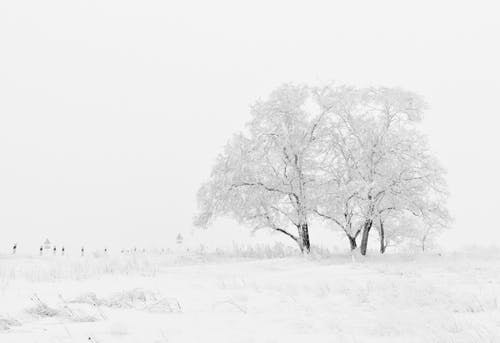
\includegraphics[width=0.3\textwidth]{snow7-pexels-photo-66284.jpeg}
  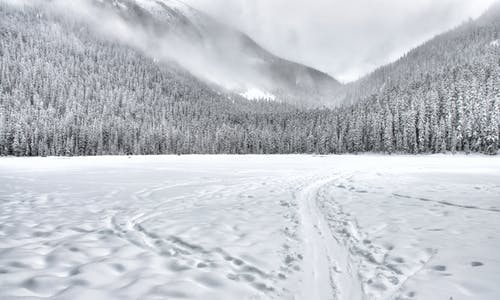
\includegraphics[width=0.3\textwidth]{snow8-pexels-photo-1571442.jpeg}
  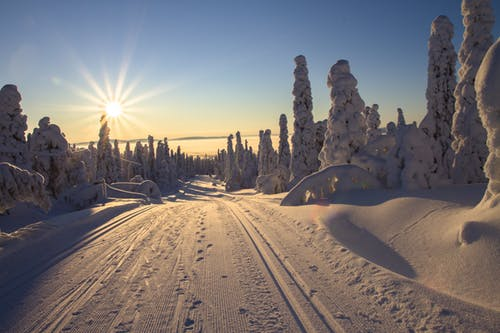
\includegraphics[width=0.3\textwidth]{snow9-pexels-photo-416728.jpeg}\
  \source{http://pexels.com}
\end{figure}

\end{frame}

%%%%%%%%%%%%%%%%%%%%%%%%%%%%%%%%%%%%
\begin{frame}{Example - which images are normal?}

\begin{figure}[ht]
  \centering
  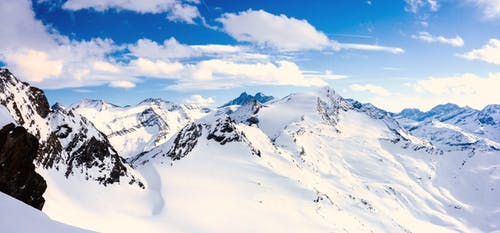
\includegraphics[width=0.3\textwidth]{test1-pexels-photo-414459.jpeg}
  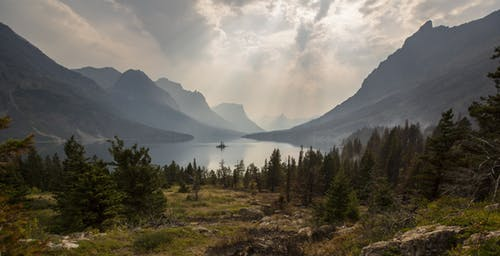
\includegraphics[width=0.3\textwidth]{test2-pexels-photo-414171.jpeg}
  \source{http://pexels.com}
\end{figure}

\end{frame}


%%%%%%%%%%%%%%%%%%%%%%%%%%%%%%%%%%%%
\begin{frame}{Application: security}

\begin{itemize}
\item Suspicious object or unusual behaviour in a scene
\end{itemize}

\begin{figure}[ht]
  \centering
  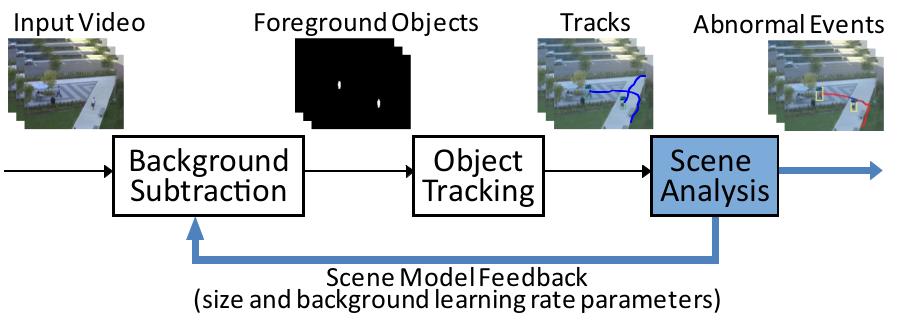
\includegraphics[width=0.8\textwidth]{motion_patterns_anom_det}
  \caption{\cite{basharat_learning_2008}}
\end{figure}


\end{frame}

%%%%%%%%%%%%%%%%%%%%%%%%%%%%%%%%%%%%
\begin{frame}{Application: industrial control}

  \begin{itemize}
  \item Fault detection
  \item Structural defect detection
   \end{itemize}

\begin{figure}[ht]
  \centering
  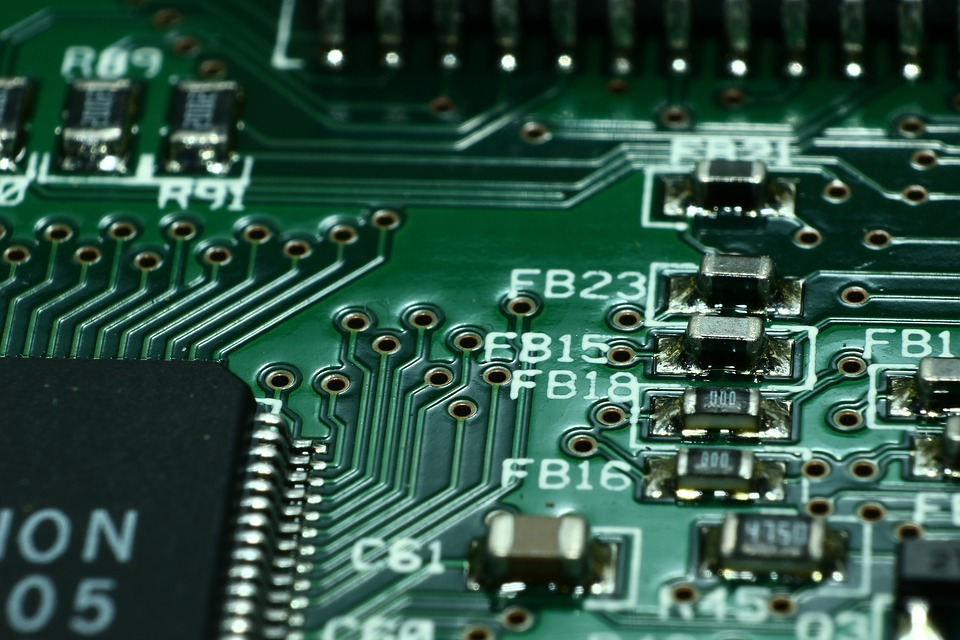
\includegraphics[width=0.5\textwidth]{printed-circuit-board-1539113_960_720.jpg}
  \source{http://www.pixabay.com}
\end{figure}


\end{frame}

%%%%%%%%%%%%%%%%%%%%%%%%%%%%%%%%%%%%
\begin{frame}{Medicine}

  \begin{itemize}
  \item Detection of suspicious conditions
  \item Non specific screening
  \end{itemize}

\begin{figure}[ht]
  \centering
  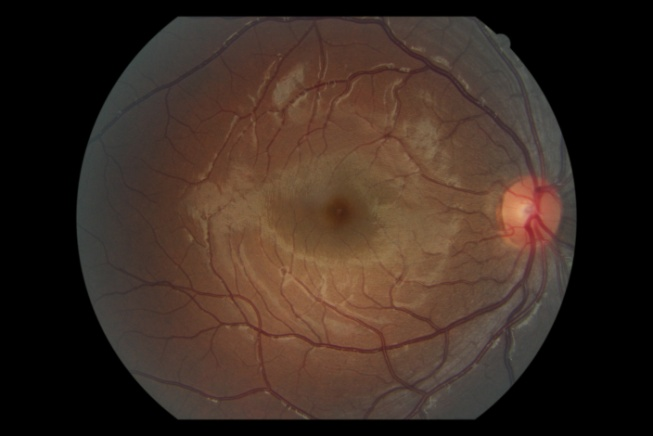
\includegraphics[width=0.5\textwidth]{fundus1}
  \caption{Retinal image used for pathology screening}
  \source{OPHDIAT database}
\end{figure}


\end{frame}


%%%%%%%%%%%%%%%%%%%%%%%%%%%%%%%%%%%%
\begin{frame}{Science}

  \begin{itemize}
  \item In some fields so many images are generated that it is becoming impossible to look at all of them
  \item Example: Euclid telescope (European Space Agency and Euclid consortium)
  \end{itemize}

  \begin{figure}[ht]
    \centering
    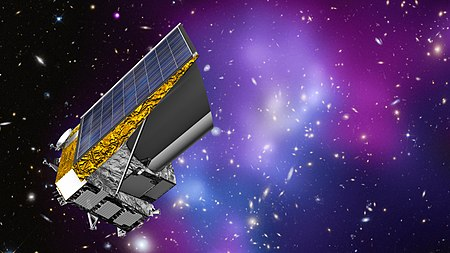
\includegraphics[width=0.5\textwidth]{450px-Euclid_ESA376594}
    \source{https://sci.esa.int/web/euclid/}
  \end{figure}


\end{frame}


%%%%%%%%%%%%%%%%%%%%%%%%%%%%%%%%%%%%
\begin{frame}{Euclid project}

\begin{itemize}
\item A new space telescope, to be launched in 2022
\item Its objective is improving our understanding of the acceleration of the universe expansion
\item To do so, the shapes of galaxies at different distances from the earth will be measured
\item An estimated $10^{10}$ extra galactic objects will be acquired by the telescope
\item Data will be automatically analyzed, without visual inspection
\end{itemize}

  \begin{figure}[ht]
    \centering
    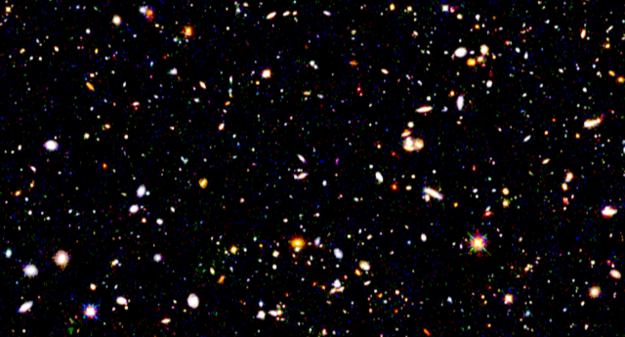
\includegraphics[width=0.5\textwidth]{ESA_Euclid_EDFF_Candels_v1_zoom_625}
    \source{https://sci.esa.int}
  \end{figure}

\end{frame}


%%%%%%%%%%%%%%%%%%%%%%%%%%%%%%%%%%%%
\begin{frame}{Anomalous images or anomalies within images?}

  \begin{itemize}
  \item When looking for anomalous images, we do not necessarily want to detect the source of the anomaly
  \item When an anomaly is detected within an image, then the image is considered as anomalous
  \end{itemize}

\end{frame}


%%%%%%%%%%%%%%%%%%%%%%%%%%%%%%%%%%%%
\begin{frame}{Vocabulary}

  \begin{itemize}
  \item Anomaly
  \item Novelty
  \item Outlier
  \end{itemize}

  In machine learning: one-class classification.
\end{frame}


%%%%%%%%%%%%%%%%%%%%%%%
%%%%%%%%%%%%%%%%%%%%%%%
\section{Mathematical modelling}

%%%%%%%%%%%%%%%%%%%%%%%%%%%%%%%%%%%%
\begin{frame}{Basic principles}

  \begin{itemize}
  \item   Let $E$ be a set (the whole set of images), $\mathcal{N}$ the subset of $E$ (constituted by all normal images) and $X$ a subset of $N$ (the set of examples that are considered to be \emph{normal}).
  \item The question we would like to answer is:

    \begin{block}{}
      \centering
    Is a given $x$ in $E$ normal?
    \end{block}

    \item What should we add to our definition of $E$, $\mathcal{N}$ and $X$ for this question to be meaningful?
  \end{itemize}

  Some possibilities:
  \begin{itemize}
  \item Metric space
  \item Probability space
  \end{itemize}

\end{frame}


%%%%%%%%%%%%%%%%%%%%%%%%%%%%%%%%%%%%
\begin{frame}{Metric space}

  $E$ is equipped with a distance $d$ such that:
  \[
  \exists d_0 \in \R^+,  \forall x \in E: x \in \mathcal{N} \iff d(x, X) \leq d_0
  \]

  Of course, the essential point will be how to choose the distance function $d$.

\end{frame}


%%%%%%%%%%%%%%%%%%%%%%%%%%%%%%%%%%%%
\begin{frame}{Probabilistic approach}

  %% In order to probabilise $E$ we need a $sigma$-algebra $\mathcal{A}$ (the events set) and a probability measure $P$.



\end{frame}



%%%%%%%%%%%%%%%%%%%%%%%%%%%%%%%%%%%%
\begin{frame}{Energy based approach}

\end{frame}


%%%%%%%%%%%%%%%%%%%%%%%%%%%%%%%%%%%%
\begin{frame}{The question of representation}

\end{frame}


%%%%%%%%%%%%%%%%%%%%%%%%%%%%%%%%%%%%%%%%%%%%%%%%%%
%%%%%%%%%%%%%%%%%%%%%%%%%%%%%%%%%%%%%%%%%%%%%%%%%%
\section{Anomaly detection using autoencoders}


%%%%%%%%%%%%%%%%%%%%%%%%%%%%%%%%%%%%
\begin{frame}{Autoencoder}

\begin{figure}[ht]
  \centering
  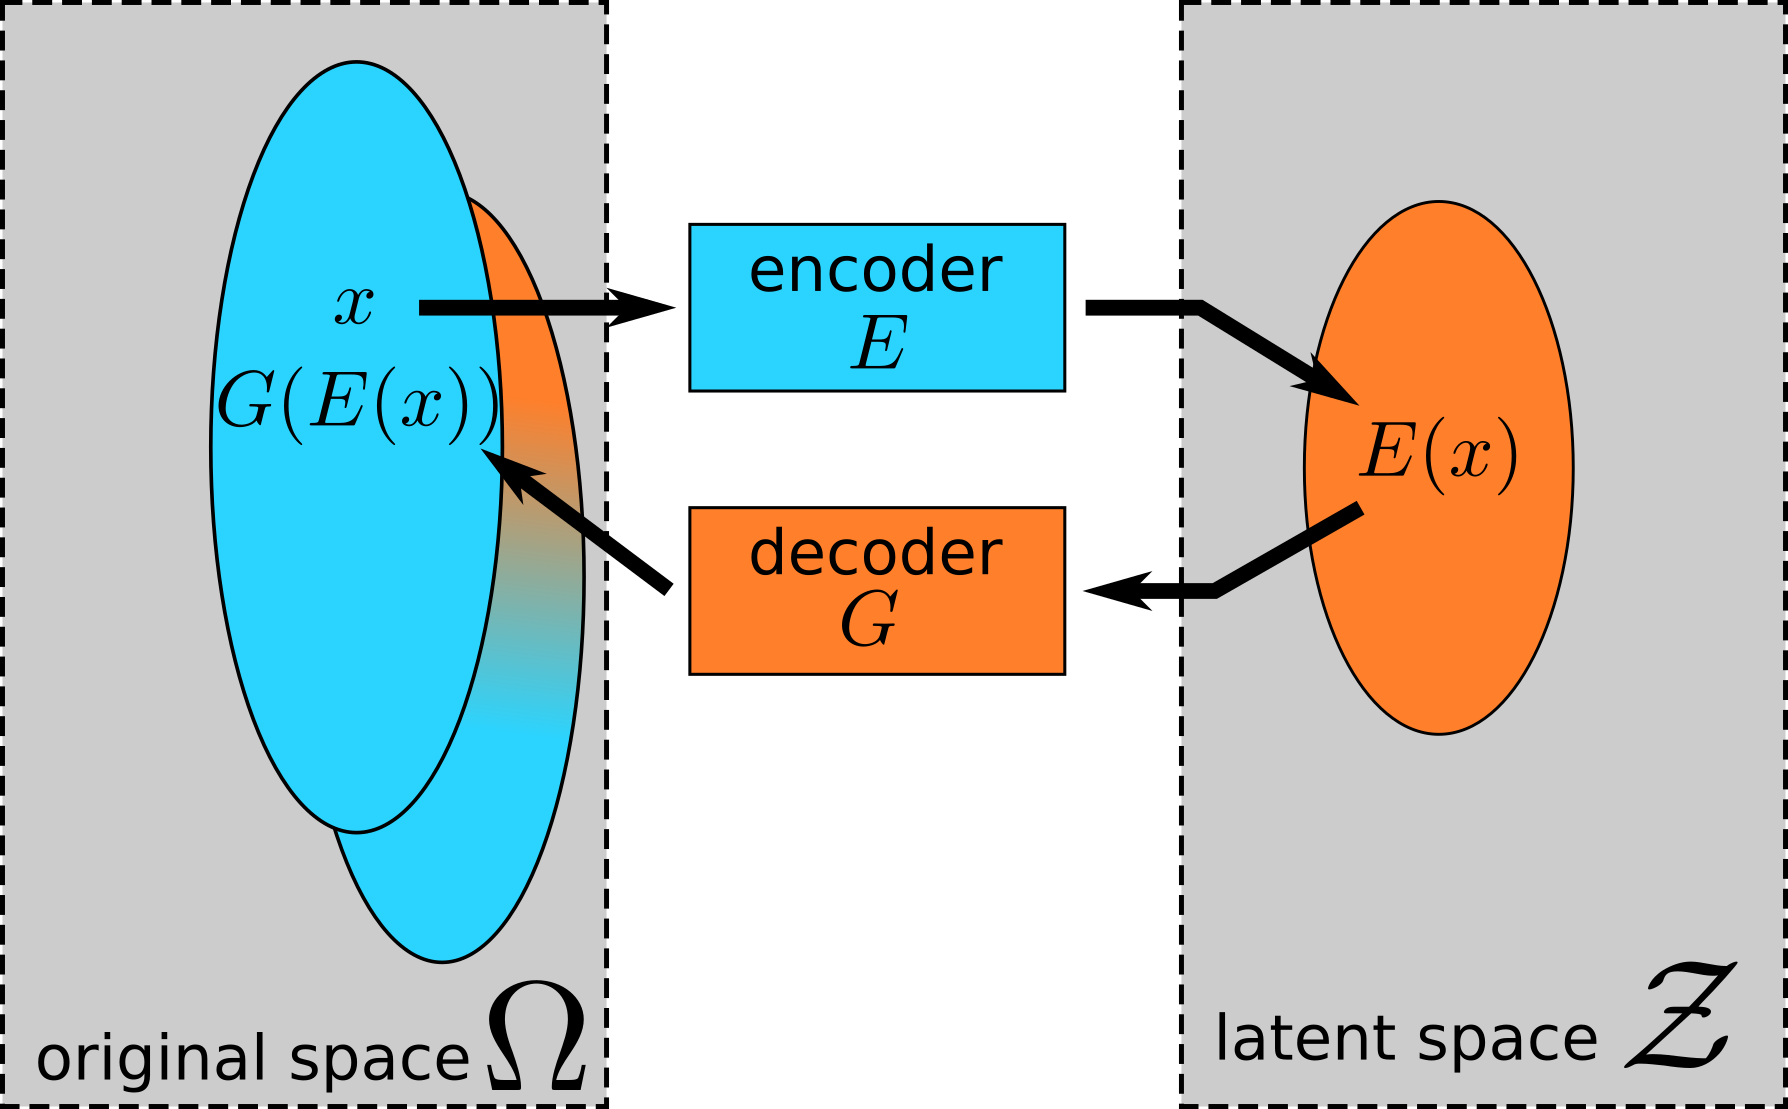
\includegraphics[width=0.5\textwidth]{ae.png}
\end{figure}

\begin{itemize}
\item Encoder: $E$; decoder: $G$; autoencoder: $G \circ E$
\item In most applications, the latent space is ``smaller'' than the data space.
  \item Objective: $\hat{x}$ ``close'' to $x$
  \item When dealing with images, modern autoencoders use convolutional neural networks
\end{itemize}

\end{frame}

%%%%%%%%%%%%%%%%%%%%%%%%%%%%%%%%%%%%
\begin{frame}{Autoencoders for anomalous image detection}

\begin{figure}[ht]
  \centering
  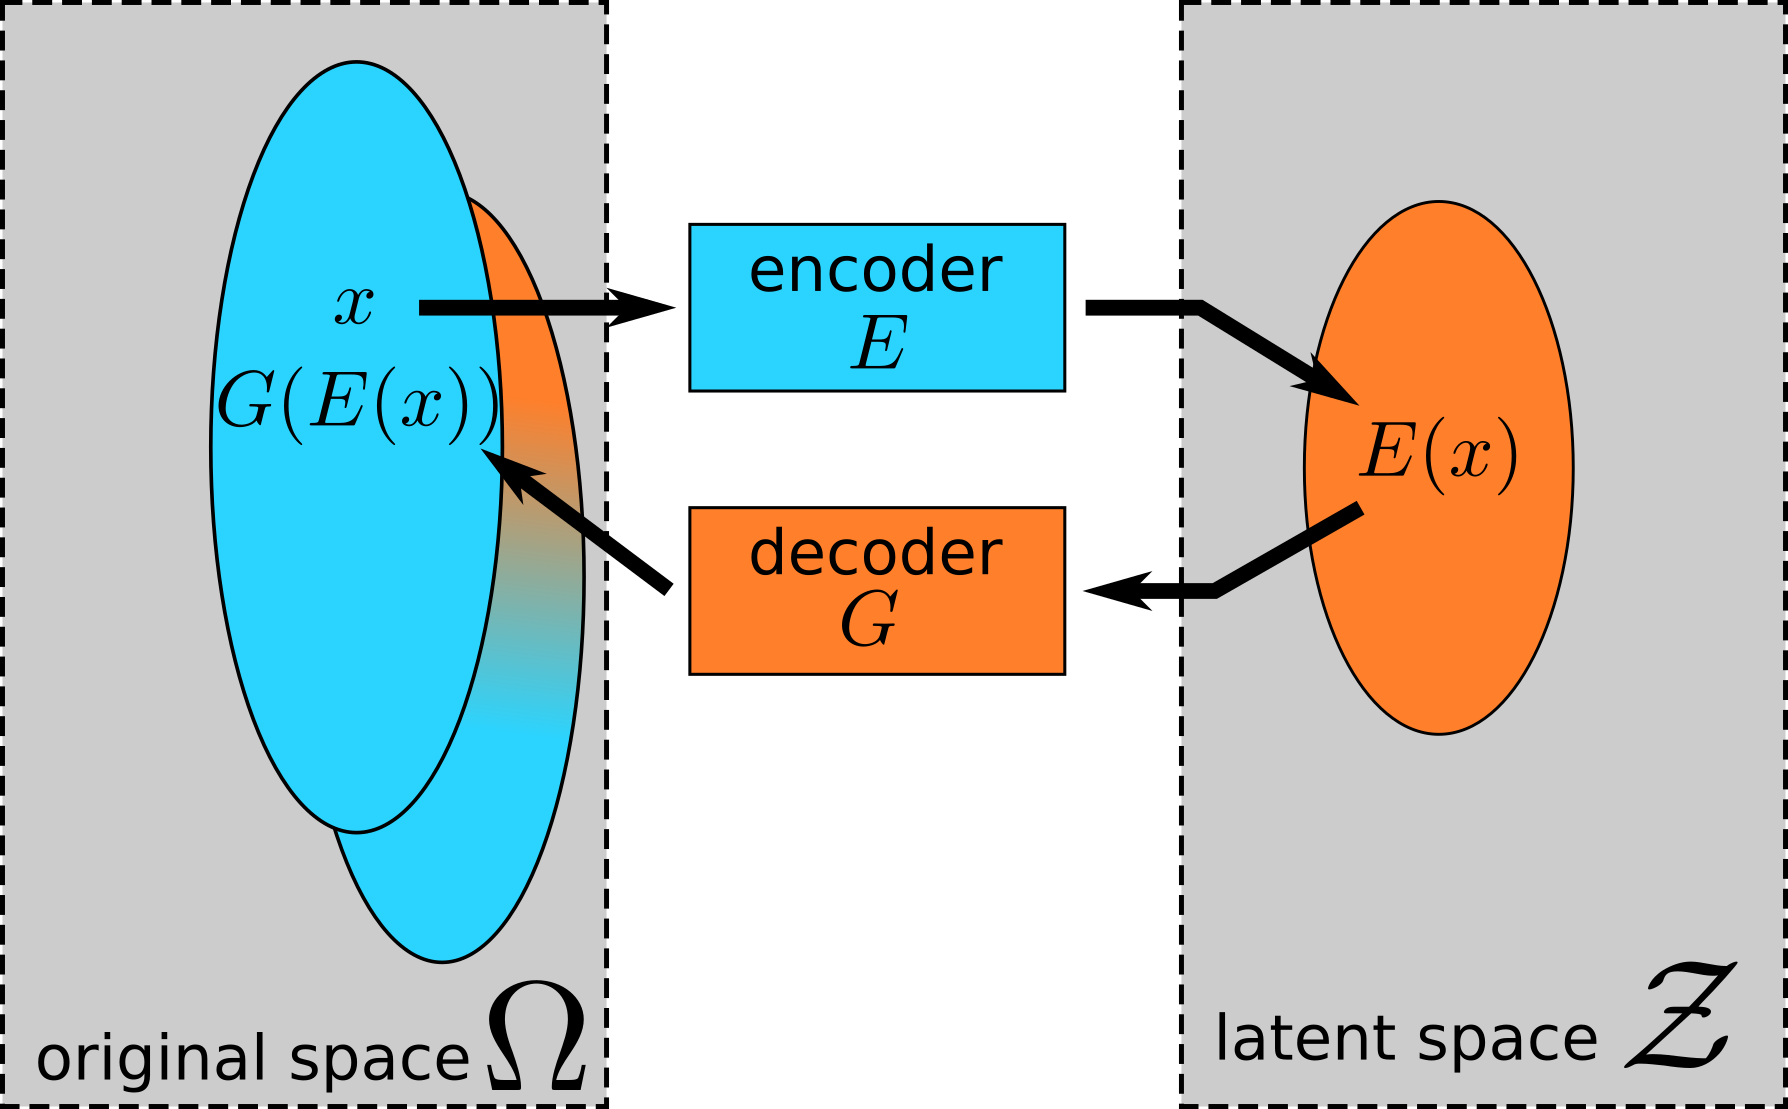
\includegraphics[width=0.5\textwidth]{ae.png}
\end{figure}

\begin{block}{Idea 1}
  The autoencoders is optimized for normal images. The coding has to be specific enough so that anomalous images are not correctly coded. The reconstruction error will therefore give a measure of the anomaly.
\end{block}

\begin{block}{Idea 2}
  The latent representation of an anomalous image should be ``far away'' from the latent representations of normal images. Image $\x$ is not normal iff $d(E(\x), E(\X)) > d_0$.
\end{block}

\end{frame}



%%%%%%%%%%%%%%%%%%%%%%%%%%%%%%%%%%%%%%%%%%%%%%%%%%
%%%%%%%%%%%%%%%%%%%%%%%%%%%%%%%%%%%%%%%%%%%%%%%%%%
\section{Anomaly detection using generative adversarial networks (GANS)}

%%%%%%%%%%%%%%%%%%%%%%%%%%%%%%%%%%%%
\begin{frame}{Generative adversarial network \cite{goodfellow_generative_2014}}

\begin{figure}[ht]
  \centering
  \includegraphics[width=0.6\textwidth]{gan2}
\end{figure}

\begin{itemize}
\item The discriminator is optimized so that it correctly classifies images as real (1) or fake (0)
  \item The generator is optimized so that the produced images are classified as real by the discriminator
\end{itemize}

\begin{block}{Value function}
$V(G,D) = \mathbb{E}_{x \sim p_{data}}(log(D(x))) + \mathbb{E}_{z \sim p_z(z)}(log(1 - D(G(z))))$
\end{block}

\end{frame}


%%%%%%%%%%%%%%%%%%%%%%%%%%%%%%%%%%%%
\begin{frame}{First application of GANs to novelty detection}

\begin{block}{Idea}
  Use the discriminator to distinguish between real and fake images.
\end{block}

\begin{itemize}
\item I have seen no mention of this strategy in the literature
\item My guess: the discriminator is not very efficient at this task. To be tested during lab sessions!
\end{itemize}

\end{frame}


%%%%%%%%%%%%%%%%%%%%%%%%%%%%%%%%%%%%
\begin{frame}{Anomaly GAN (AnoGAN) \cite{schlegl_unsupervised_2017}}

\begin{figure}[ht]
  \centering
  \includegraphics[width=0.6\textwidth]{gan2}
\end{figure}

\begin{enumerate}
\item Learn a GAN on the set of normal images
\item For a new image $\x$ (normal or not):
  \begin{itemize}
  \item Find a $z^*$ such that $G(z^*)$ is \emph{close as possible} to $\x$
  \item If $G(z^*)$ is \emph{similar enough} to $\x$ and is \emph{correctly evaluated by the descriminator}, then $\x$ is considered as normal
  \end{itemize}
\end{enumerate}

\end{frame}

%%%%%%%%%%%%%%%%%%%%%%%%%%%%%%%%%%%%
\begin{frame}{Find $z^*$}

  \begin{figure}[ht]
  \centering
  \includegraphics[width=0.6\textwidth]{gan2}
\end{figure}



\end{frame}


%%%%%%%%%%%%%%%%%%%%%%%%%%%%%%%%%%%%
\begin{frame}{Is $\x$ similar to $G(z^*)$ ?}

\begin{figure}[ht]
  \centering
  \includegraphics[width=0.6\textwidth]{gan2}
\end{figure}

\begin{block}{Residual loss}
  \centering
  $\mathcal{L}_R(z^*) = \norm{x - G(z^*)}_{L_1}$
  \end{block}

\end{frame}


%%%%%%%%%%%%%%%%%%%%%%%%%%%%%%%%%%%%
\begin{frame}{Is $G(z^*)$ realistic?}

\begin{figure}[ht]
  \centering
  \includegraphics[width=0.6\textwidth]{gan2}
\end{figure}

\begin{block}{Discrimination loss}
  \centering
  $\mathcal{L}_D(z^*) = D(G(z^*))$
\end{block}

\begin{block}{Improved discrimination loss}
  \[\mathcal{L}_D(z^*) = \norm{E(x) -  E(D(G(z^*)))}_{L_1}\]
  where $f$ is the an intermediate layer of the discriminator.
\end{block}


\end{frame}


%%%%%%%%%%%%%%%%%%%%%%%%%%%%%%%%%%%%
\begin{frame}{Example (from \cite{schlegl_unsupervised_2017})}


  \begin{figure}[ht]
    \centering
    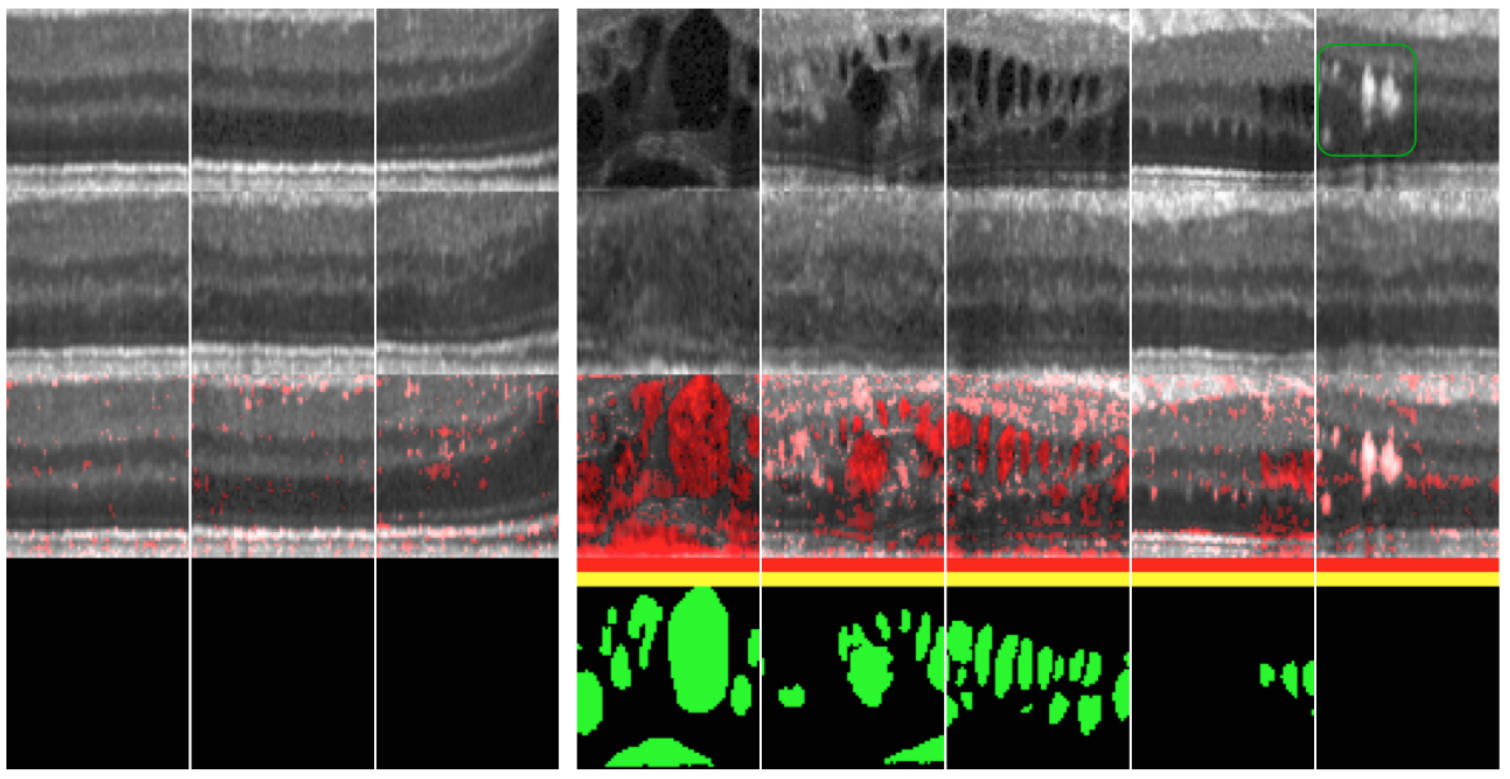
\includegraphics[width=\textwidth]{res_oct}
    \caption{Left block: normal OCT sections, from test set. Right block: anomalous OCT sections; bottom line: expert annotation of retinal fluid}
  \end{figure}

\end{frame}


%%%%%%%%%%%%%%%%%%%%%%%%%%%%%%%%%%%%
\begin{frame}{AnoGAN improvement}

\begin{figure}[ht]
  \centering
  \includegraphics[width=0.6\textwidth]{gan2}
\end{figure}

\begin{itemize}
\item For a given real image $\x$, finding a latent code $z$ such that $D(z)$ is similar to $x$ is computationally intensive
\item Idea: learn an encoder to compute $z$ from $\x$
\end{itemize}

\end{frame}

%%%%%%%%%%%%%%%%%%%%%%%%%%%%%%%%%%%%
\begin{frame}{BiGAN}

\begin{figure}[ht]
  \centering
  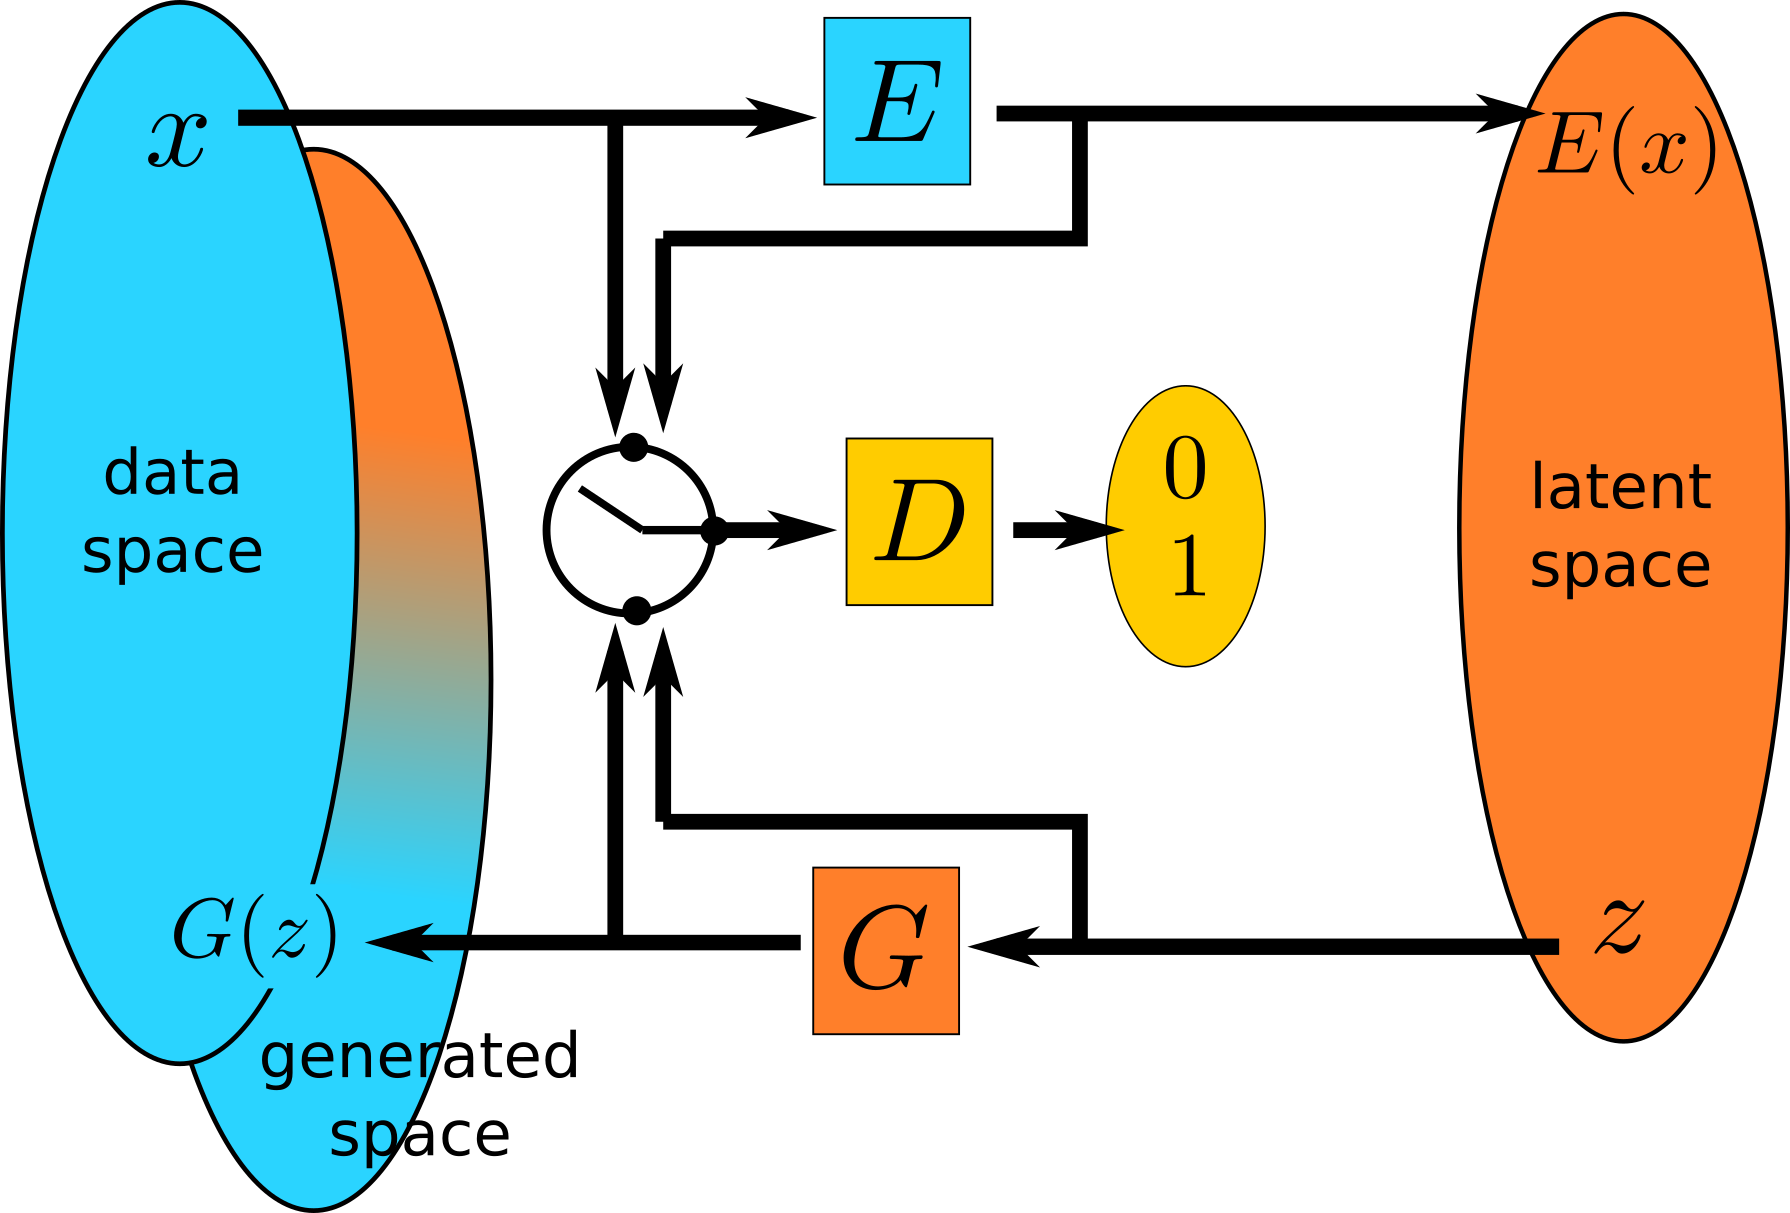
\includegraphics[width=0.6\textwidth]{bigan}
\end{figure}

\begin{itemize}
\item An encoder is added to the architecture
\item The discriminator takes as input pairs of image / code
\end{itemize}


\end{frame}

%%%%%%%%%%%%%%%%%%%%%%%%%%%%%%%%%%%%
\begin{frame}{BiGAN: application to novelty detection}

\begin{figure}[ht]
  \centering
  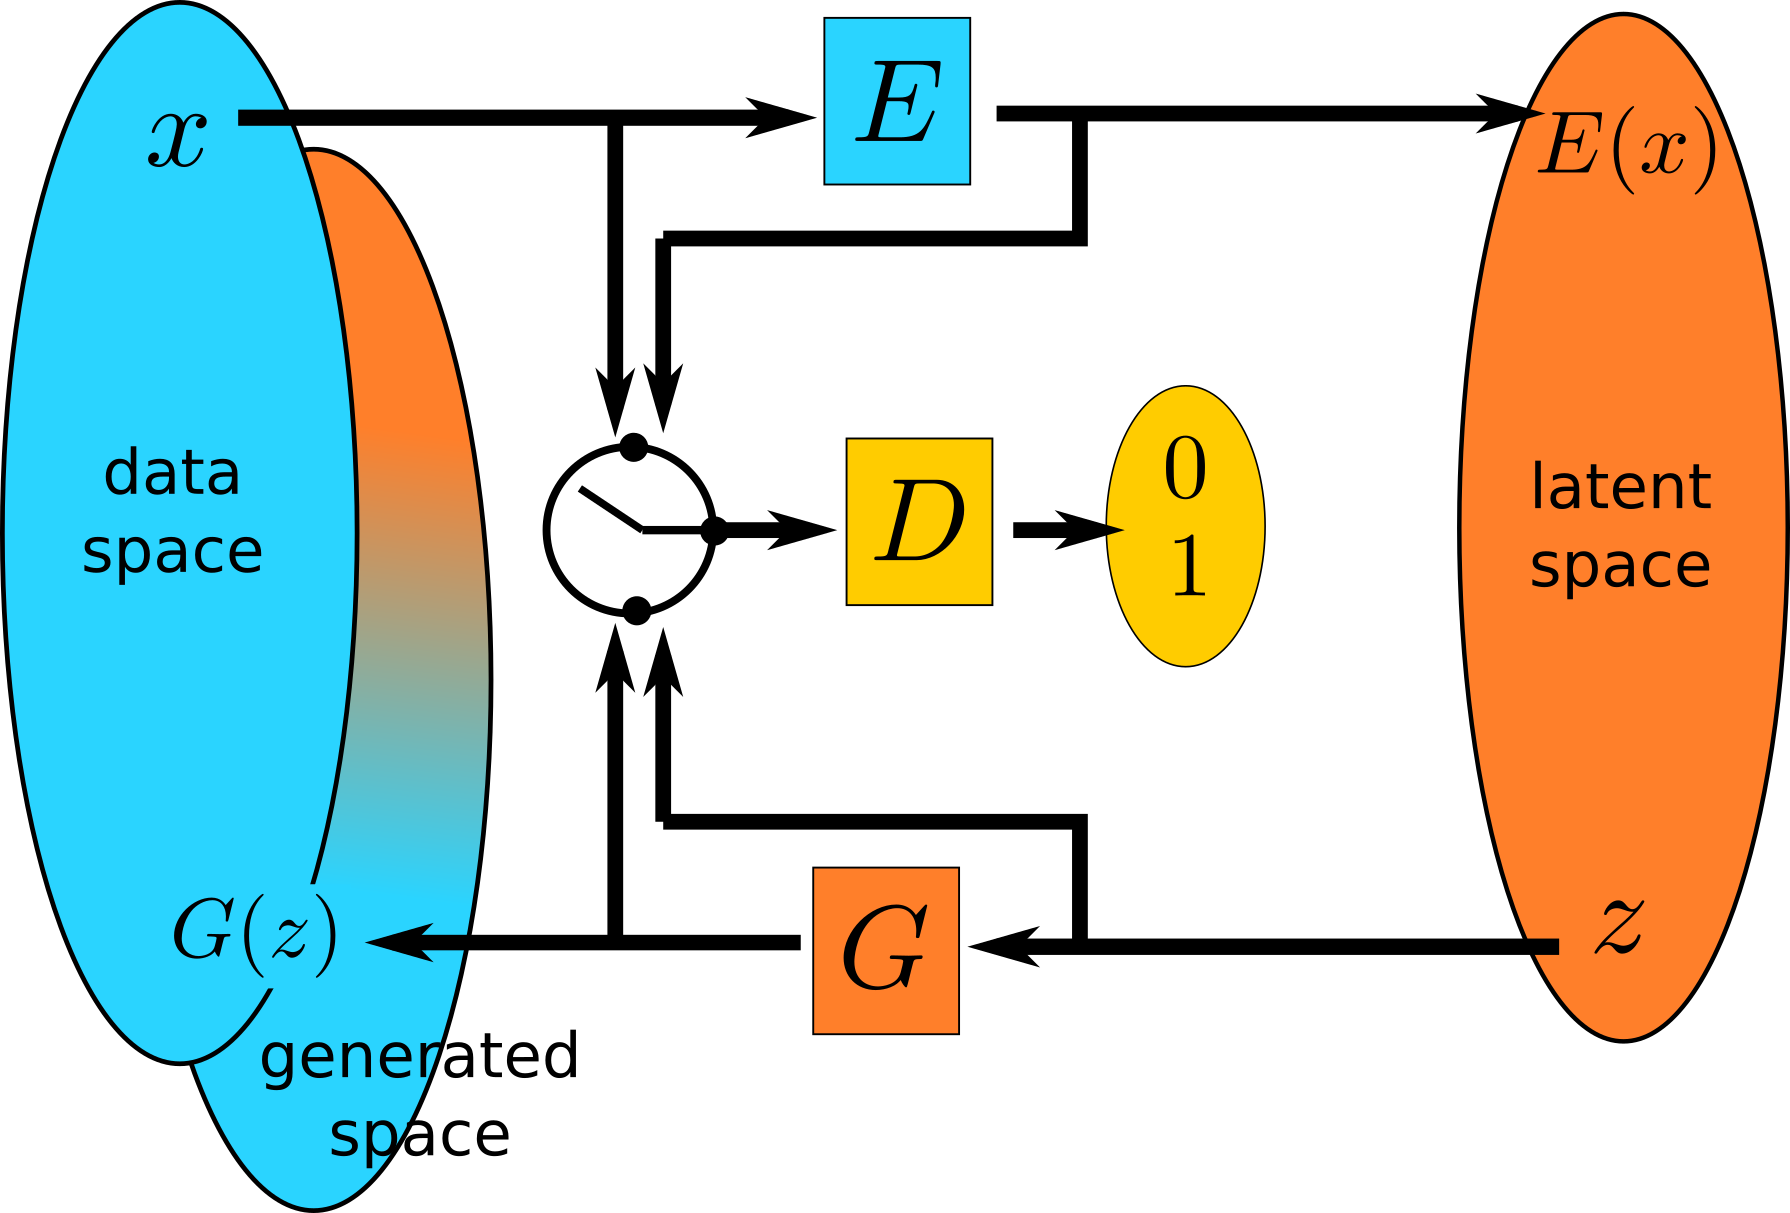
\includegraphics[width=0.6\textwidth]{bigan}
\end{figure}

\begin{itemize}
\item Similar to AnoGAN, except that looking for a convenient $z^*$ for a given real image $x$ is done using the encoder $E$
\item Better anomaly detection results on MNIST
\item Much faster (800x)
\end{itemize}


\end{frame}



%%%%%%%%%%%%%%%%%%%%%%%%%%%%%%%%%%%%%%%%%%%%%%%%%%
\section*{References}

%%%%%%%%%%%%%%%%%%%%%%%%%%%%%%%%%%%%%%%%%%%%%%%%%%

\frame[allowframebreaks]{

  \scriptsize

  \frametitle{References}

  %\bibliographystyle{amsalpha}
  %\bibliographystyle{apalike}

  \bibliography{../../edf.bib}

  \normalsize

}




\end{document}
